\documentclass[conference]{IEEEtran}

\usepackage{amsmath,amssymb,amsfonts}
\usepackage{graphicx}
\usepackage{textcomp}
\usepackage{xcolor}
\usepackage{booktabs}
\usepackage{array}
\usepackage{listings}
\usepackage{url}
\usepackage{hyperref}
\usepackage{cite}
\hypersetup{hidelinks}

% Code Listing Style
\lstset{
	language=Python,
	basicstyle=\ttfamily\footnotesize,
	keywordstyle=\color{blue}\bfseries,
	commentstyle=\color{gray}\itshape,
	stringstyle=\color{red},
	numbers=left,
	numberstyle=\tiny\color{gray},
	numbersep=5pt,
	frame=single,
	breaklines=true,
	captionpos=b,
	tabsize=4
}

\def\BibTeX{{\rm B\kern-.05em{\sc i\kern-.025em b}\kern-.08em
		T\kern-.1667em\lower.7ex\hbox{E}\kern-.125emX}}

\begin{document}
	
	\title{Predicting Customer Churn in the Telecommunications Industry: A Comparative Study of Classification Algorithms\\
		{\footnotesize BIL 476 --- Data Mining Course Project, Summer 2026\\
			TOBB University of Economics and Technology}
	}
	
	\author{\IEEEauthorblockN{Zeynep Ay}
		\IEEEauthorblockA{\textit{TOBB University of Economics and Technology}\\
			Ankara, Turkey \\
			Student ID: 231404035 \\
			\href{mailto:zay@etu.edu.tr}{zay@etu.edu.tr}}
	}
	
	\maketitle
	
	\begin{abstract}
	Customer churn is a costly problem for telecommunications companies because replacing customers generally requires more resources than retaining them. This project predicts churn from account, service, and billing attributes using the public IBM Telco Customer Churn dataset. The dataset contains 7{,}043 customer records, 19 predictive attributes of mixed nominal and numeric types, and a binary churn target. Data cleaning revealed 11 blank values hidden in the \texttt{TotalCharges} field and a class imbalance of 73.5\% retained customers versus 26.5\% churned customers. Four classifiers---Decision Tree, Gaussian Naive Bayes, k-Nearest Neighbors, and Random Forest---were tuned with stratified five-fold cross-validation and evaluated on an untouched 20\% test set. Preprocessing was fitted within each cross-validation fold to prevent leakage. Baseline models were compared with variants using SMOTENC, which respects the dataset's mixed categorical and numeric feature types. The best baseline accuracy was 80.3\%, achieved by Random Forest, which also produced the highest ROC-AUC (0.839) and PR-AUC (0.653). Random Forest with SMOTENC achieved the highest F1-score (0.605), with 67.4\% recall and 54.9\% precision. Naive Bayes with SMOTENC produced a similar F1-score (0.603) with higher recall (77.8\%) but lower precision (49.2\%). These results show that the preferred model depends on whether a retention campaign prioritizes detecting more churners or limiting false alarms.
	\end{abstract}
	
	\begin{IEEEkeywords}
		data mining, customer churn, classification, telecommunications, class imbalance
	\end{IEEEkeywords}
	
	\section{Introduction}
	\label{sec:introduction}
	
	Customer churn occurs when a customer stops using a company's service. It is an important problem for telecommunications companies because attracting a new customer generally costs more than keeping an existing one~\cite{b2}. If customers who are likely to leave can be identified early, a company can direct retention offers to those customers instead of applying the same campaign to everyone.
	
	This project asks how accurately customer churn can be predicted from account, service, and billing information, and how different classifiers behave when the churn class is smaller than the non-churn class. We compare Decision Tree, Gaussian Naive Bayes, k-Nearest Neighbors (k-NN), and Random Forest on the IBM Telco Customer Churn dataset. The algorithms use different learning strategies, allowing their predictive performance and practical trade-offs to be compared.
	
	The remainder of this paper is organized as follows. Section~\ref{sec:related_work} reviews related work on customer churn prediction. Section~\ref{sec:dataset} describes the dataset and its characteristics. Section~\ref{sec:methodology} details the data preprocessing pipeline, the algorithms used, and the experimental setup. Section~\ref{sec:results} presents the experimental results. Section~\ref{sec:discussion} discusses the findings, limitations, and ethical considerations. Section~\ref{sec:conclusion} concludes the paper and outlines directions for future work.
	
	\section{Related Work}
	\label{sec:related_work}
	
	Predicting customer churn in telecommunications has been studied with many classification methods. Ahmad et al.~\cite{b1} used data from a Syrian telecom operator and compared Decision Tree, Random Forest, Gradient Boosted Machine, and XGBoost. XGBoost gave their strongest result, and the study also emphasized the low proportion of churn customers. Mustafa et al.~\cite{b2} compared six classifiers on data from a Malaysian telecom operator; among their tested methods, CART achieved the highest accuracy. Sana et al.~\cite{b3} evaluated eight algorithms with several data-transformation methods across four public telecom datasets and found improvements from combining transformations with ensemble classifiers.

	Wagh et al.~\cite{b5} also compared multiple machine-learning classifiers for telecom churn and reported strong performance from ensemble tree methods. Chang et al.~\cite{b6} combined churn classifiers with SHAP and LIME to examine the variables influencing predictions. These studies show that model comparison, class imbalance, and interpretability are recurring concerns in churn prediction. Chawla et al.~\cite{b4} introduced SMOTE for minority-class oversampling. This project uses SMOTENC, its mixed-data extension, so categorical variables are handled as categories during sample generation.
	
	This project has a narrower objective. Instead of trying to obtain the highest possible score with many transformations or advanced models, it provides a reproducible baseline comparison of four common classifiers on one public dataset. Each classifier is evaluated both with the original training distribution and with SMOTENC, making the effect of imbalance handling easier to observe.
	
	\section{Dataset Description}
	\label{sec:dataset}
	
	\subsection{Data Source}
	The IBM Telco Customer Churn dataset was originally released as IBM sample data and is available on Kaggle~\cite{b7,b8}. The verified Kaggle page is \url{https://www.kaggle.com/datasets/blastchar/telco-customer-churn}. It represents a fictional telecommunications company and records each customer's demographic information, subscribed services, contract and billing information, and whether the customer churned. The dataset was selected because it represents a clear classification problem, contains both nominal and numeric attributes, and is small enough to reproduce on a standard computer.
	
	\subsection{Data Characteristics}
	Table~\ref{tab:dataset} summarizes the key properties of the dataset.
	
	\begin{table}[htbp]
		\caption{Dataset Summary}
		\begin{center}
			\resizebox{\columnwidth}{!}{%
			\begin{tabular}{|l|l|}
				\hline
				\textbf{Property} & \textbf{Value} \\
				\hline
				Number of Records & 7{,}043 \\
				\hline
				Number of Predictive Attributes & 19 (customer ID excluded) \\
				\hline
				Attribute Types & 16 Nominal, 3 Numeric \\
				\hline
				Target Variable & Churn (Yes / No) \\
				\hline
				Missing / Invalid Values & 11 records (0.16\%) with a blank \\
				& \texttt{TotalCharges} value (all with \\
				& tenure = 0); corrected during \\
				& preprocessing (Section~\ref{sec:methodology}) \\
				\hline
				Class Distribution & 73.5\% No-Churn / 26.5\% Churn \\
				\hline
				Source URL & kaggle.com/datasets/blastchar/ \\
				& telco-customer-churn \\
				\hline
			\end{tabular}}
			\label{tab:dataset}
		\end{center}
	\end{table}
	
	The three numeric attributes are \texttt{tenure} (number of months the customer has stayed with the company), \texttt{MonthlyCharges}, and \texttt{TotalCharges}. Table~\ref{tab:numstats} reports descriptive statistics for these attributes computed on the cleaned dataset.
	
	\begin{table}[htbp]
		\caption{Descriptive Statistics for Numeric Attributes}
		\begin{center}
			\resizebox{\columnwidth}{!}{%
			\begin{tabular}{|l|c|c|c|c|}
				\hline
				\textbf{Attribute} & \textbf{Mean} & \textbf{Std.} & \textbf{Min} & \textbf{Max} \\
				\hline
				tenure (months) & 32.37 & 24.56 & 0 & 72 \\
				\hline
				MonthlyCharges (\$) & 64.76 & 30.09 & 18.25 & 118.75 \\
				\hline
				TotalCharges (\$) & 2279.73 & 2266.79 & 0.00 & 8684.80 \\
				\hline
			\end{tabular}}
			\label{tab:numstats}
		\end{center}
	\end{table}
	
	The 16 nominal attributes include demographic fields (\texttt{gender}, \texttt{SeniorCitizen}, \texttt{Partner}, \texttt{Dependents}), service-subscription fields (\texttt{PhoneService}, \texttt{MultipleLines}, \texttt{InternetService}, \texttt{OnlineSecurity}, \texttt{OnlineBackup}, \texttt{DeviceProtection}, \texttt{TechSupport}, \texttt{StreamingTV}, \texttt{StreamingMovies}), and account fields (\texttt{Contract}, \texttt{PaperlessBilling}, \texttt{PaymentMethod}).
	
	\subsection{Ethical Considerations}
	The dataset is public sample data and does not contain customer names or addresses. Its \texttt{customerID} field is an anonymized identifier and was removed before modeling. However, the dataset includes demographic attributes such as \texttt{gender} and \texttt{SeniorCitizen}. If a churn model were used in practice, its errors should therefore be compared across customer groups before it is used to guide retention decisions. Feature importance alone cannot prove that a model is fair. Both ChatGPT and Claude were used during this project for coding, debugging, and pipeline improvement. The student prepared the initial report outline, section structure, and content plan; ChatGPT then assisted with developing parts of the report, language revision, structural refinement, and LaTeX formatting. Only this public dataset was used; no private or confidential customer data was shared with these AI tools.
	
	\section{Methodology}
	\label{sec:methodology}
	
	\subsection{Data Preprocessing}
	The following preprocessing steps were applied to the raw dataset:
	\begin{itemize}
		\item \textbf{Missing/invalid value handling:} Although a naive null check reports zero missing values, 11 records store an empty string in the \texttt{TotalCharges} field instead of a numeric value. These records were identified by converting the column to a numeric type and inspecting the resulting missing values. All 11 correspond to customers with \texttt{tenure} = 0, i.e. brand-new customers who have not yet been billed; these values were therefore imputed as 0 rather than with a summary statistic such as the mean, since 0 is the value that is actually consistent with these customers' billing history.
		\item \textbf{Identifier removal:} The \texttt{customerID} column was removed, since it is a unique identifier with no predictive value and its inclusion would risk data leakage or spurious memorization.
		\item \textbf{Consistency recoding:} The \texttt{SeniorCitizen} attribute, originally encoded as 0/1, was recoded to Yes/No to be consistent with the representation of the dataset's other binary nominal attributes.
		\item \textbf{Target encoding:} The target variable \texttt{Churn} (Yes/No) was additionally encoded as a binary indicator (\texttt{Churn\_binary}, 1 = Yes) to support both the descriptive analysis in Section~\ref{sec:dataset} and downstream model training.
	\end{itemize}
	Categorical attributes were one-hot encoded, while the three continuous attributes (\texttt{tenure}, \texttt{MonthlyCharges}, and \texttt{TotalCharges}) were standardized for k-NN because distance-based models are sensitive to feature scale. Encoding and scaling were implemented as pipeline steps fitted separately within each cross-validation training fold. This prevents validation-fold statistics from leaking into model training. Decision Tree, Naive Bayes, and Random Forest received unscaled numeric features. To evaluate class-imbalance handling, each baseline model was compared with a SMOTENC variant. SMOTENC was also placed inside the cross-validation pipeline, so synthetic samples were generated only from each training fold and categorical attributes were handled explicitly as categorical rather than interpolated as one-hot values.
	
	\subsection{Algorithm Selection and Description}
	Four classification algorithms were selected to compare a range of modeling assumptions, from simple and interpretable to ensemble-based:
	\begin{itemize}
		\item \textbf{Decision Tree:} A recursive, rule-based classifier that splits the feature space based on information-theoretic criteria such as Gini impurity or entropy. It was selected for its interpretability: the resulting tree structure can be read directly by a non-technical stakeholder as a set of ``if-then'' retention rules.
		\item \textbf{Naive Bayes:} A probabilistic classifier based on Bayes' theorem under a (naive) conditional independence assumption between features. It was selected as a computationally inexpensive baseline that is known to perform competitively on datasets with largely categorical attributes, as in~\cite{b2}.
		\item \textbf{k-Nearest Neighbors (k-NN):} An instance-based, non-parametric classifier that assigns the majority class among the $k$ nearest training examples. It was selected because it can capture local patterns in the preprocessed feature space.
		\item \textbf{Random Forest:} An ensemble of decision trees trained on bootstrap samples with random feature subsets, combined via majority voting. It was selected because ensemble methods have consistently outperformed single classifiers in the churn-prediction literature reviewed in Section~\ref{sec:related_work}~\cite{b1,b3}, while still allowing feature importance to be extracted for interpretability.
	\end{itemize}
	Together, these algorithms allow models with different levels of complexity and interpretability to be compared.
	
	\subsection{Experimental Setup}
	\begin{itemize}
		\item \textbf{Train/test split:} 80\% / 20\% stratified split, preserving the 73.5\%/26.5\% class ratio in both subsets.
		\item \textbf{Hyperparameter selection:} Key hyperparameters (e.g., tree depth for Decision Tree and Random Forest and $k$ for k-NN) were selected by stratified 5-fold cross-validation on the training set, optimizing churn-class F1-score. Baseline and SMOTENC variants were tuned separately.
		\item \textbf{Software environment:} Python 3.10, with pandas and NumPy for data handling, scikit-learn and imbalanced-learn for model training and evaluation, and matplotlib/seaborn for visualization.
		\item \textbf{Hardware:} Standard consumer-grade hardware (CPU only); no specialized hardware is required given the dataset size.
	\end{itemize}
	
	\subsection{Reproducibility and Verification}
	All preprocessing and modeling steps are implemented in Jupyter notebooks. A fixed random seed (\texttt{random\_state=42}) is used for the train/test split, cross-validation, SMOTENC, and stochastic classifiers. The GitHub repository contains the notebooks, dependency list, dataset link, generated results, and execution instructions. The notebooks were run in the stated order and the reported tables were checked against the exported results file.
	
	\section{Results}
	\label{sec:results}
	
	All four algorithms were trained both on the original imbalanced training data and with SMOTENC inside their cross-validation pipelines. The selected models were then evaluated once on the same held-out, untouched 20\% test set (1{,}409 customers), which retained the real-world 73.5\%/26.5\% class ratio.
	
	\subsection{Evaluation Metrics}
	Because the target class is imbalanced (73.5\%/26.5\%), accuracy alone would be misleading: a trivial classifier that always predicts ``No Churn'' would achieve 73.5\% accuracy while never identifying a churner. We therefore report Accuracy, Precision, Recall, F1-score, ROC-AUC, and PR-AUC for each model. PR-AUC is particularly informative here because it focuses on the precision--recall trade-off for the minority class. Recall and F1-score are emphasized because failing to identify a customer who will churn may be more costly to a retention program than incorrectly flagging a loyal customer.
	
	\subsection{Results Summary}
	Table~\ref{tab:results} reports test-set performance for all eight model variants (four baseline and four SMOTENC-trained), sorted by F1-score.
	
	\begin{table}[htbp]
		\caption{Test-Set Performance, Sorted by F1-score}
		\label{tab:results}
		\begin{center}
			\scriptsize
			\resizebox{\columnwidth}{!}{%
			\begin{tabular}{|l|c|c|c|c|c|c|}
				\hline
				\textbf{Model} & \textbf{Acc.} & \textbf{Prec.} & \textbf{Rec.} & \textbf{F1} & \textbf{ROC} & \textbf{PR} \\
				\hline
				Random Forest (SMOTENC) & 0.767 & 0.549 & 0.674 & \textbf{0.605} & 0.830 & 0.616 \\
				\hline
				Naive Bayes (SMOTENC) & 0.728 & 0.492 & 0.778 & 0.603 & 0.804 & 0.575 \\
				\hline
				k-NN (SMOTENC) & 0.730 & 0.495 & 0.762 & 0.600 & 0.808 & 0.560 \\
				\hline
				Decision Tree & 0.798 & 0.635 & 0.567 & 0.599 & 0.828 & 0.621 \\
				\hline
				Naive Bayes & 0.703 & 0.465 & \textbf{0.810} & 0.591 & 0.819 & 0.603 \\
				\hline
				Decision Tree (SMOTENC) & 0.728 & 0.492 & 0.738 & 0.590 & 0.791 & 0.499 \\
				\hline
				Random Forest & \textbf{0.803} & \textbf{0.662} & 0.524 & 0.585 & \textbf{0.839} & \textbf{0.653} \\
				\hline
				k-NN & 0.780 & 0.589 & 0.564 & 0.577 & 0.827 & 0.601 \\
				\hline
			\end{tabular}}
		\end{center}
	\end{table}
	
	\subsection{Visualizations}

	Figures~\ref{fig:f1comparison}--\ref{fig:featimportance} provide complementary views of the results. They compare F1-scores, ROC curves, precision--recall curves, and confusion matrices for the evaluated variants. The final figure reports the feature importance values produced by the baseline Random Forest model.
	
	\begin{figure}[htbp]
		\centering
		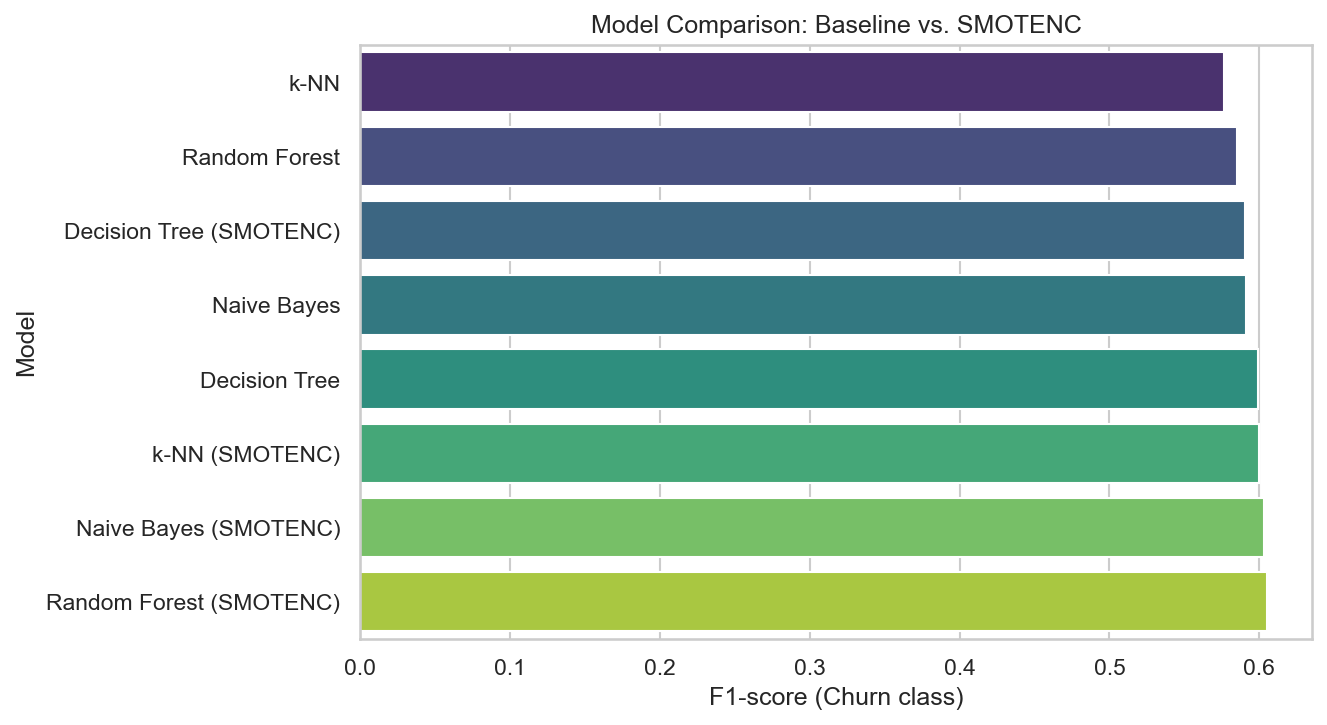
\includegraphics[width=0.48\textwidth]{figures_f1_comparison.png}
		\caption{F1-score comparison across all eight model variants.}
		\label{fig:f1comparison}
	\end{figure}
	
	\begin{figure}[htbp]
		\centering
		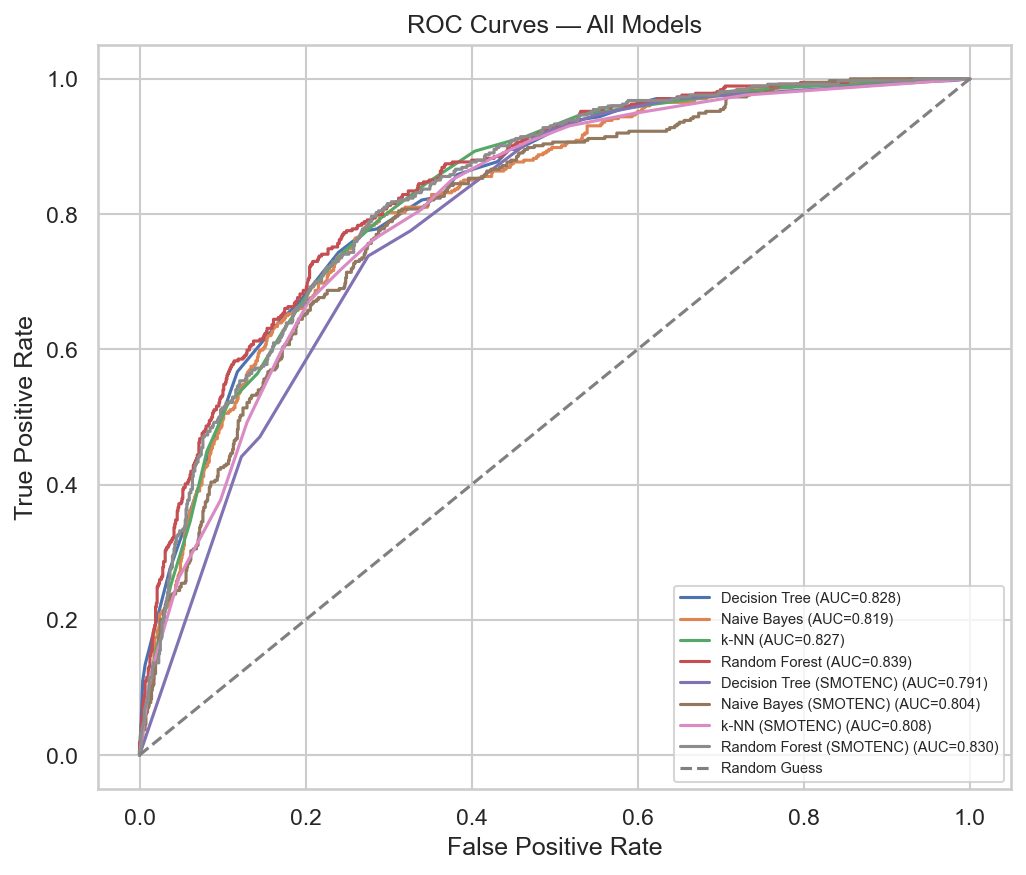
\includegraphics[width=0.48\textwidth]{figures_roc_curves.png}
		\caption{ROC curves for all eight baseline and SMOTENC-trained model variants.}
		\label{fig:roccurves}
	\end{figure}
	
	\begin{figure}[htbp]
		\centering
		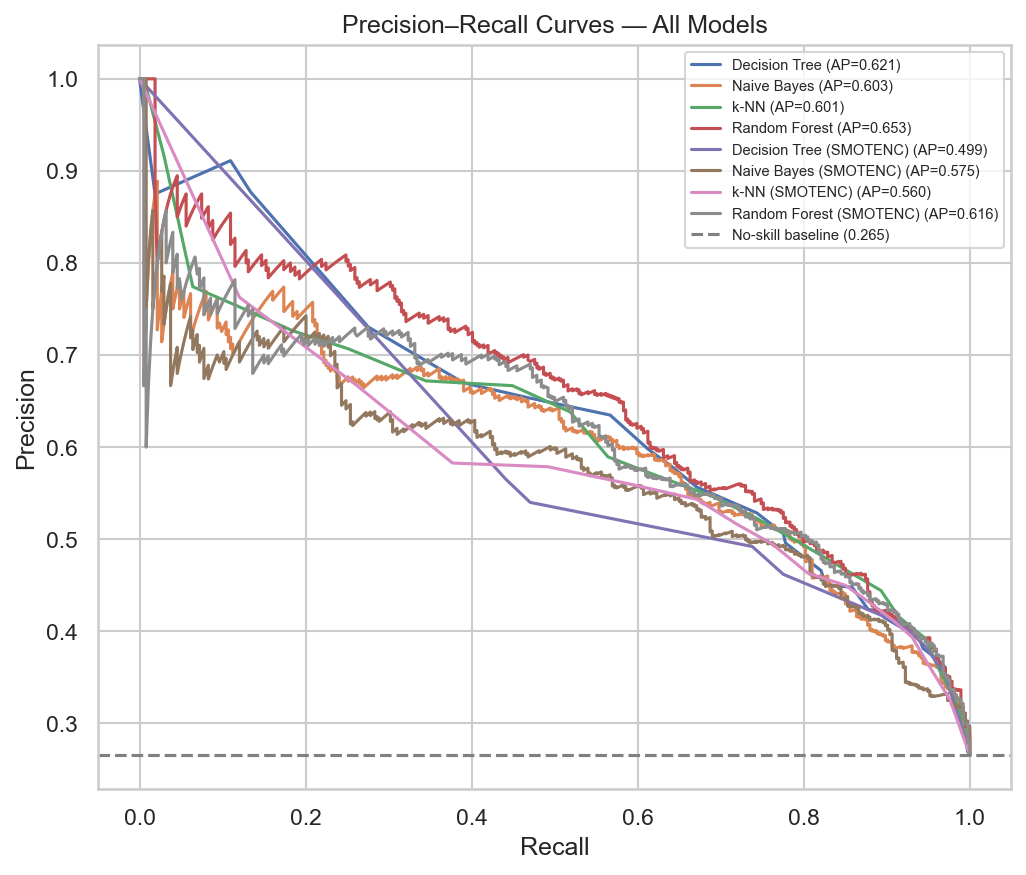
\includegraphics[width=0.48\textwidth]{figures_pr_curves.png}
		\caption{Precision--recall curves for all eight model variants.}
		\label{fig:prcurves}
	\end{figure}
	
	\begin{figure}[htbp]
		\centering
		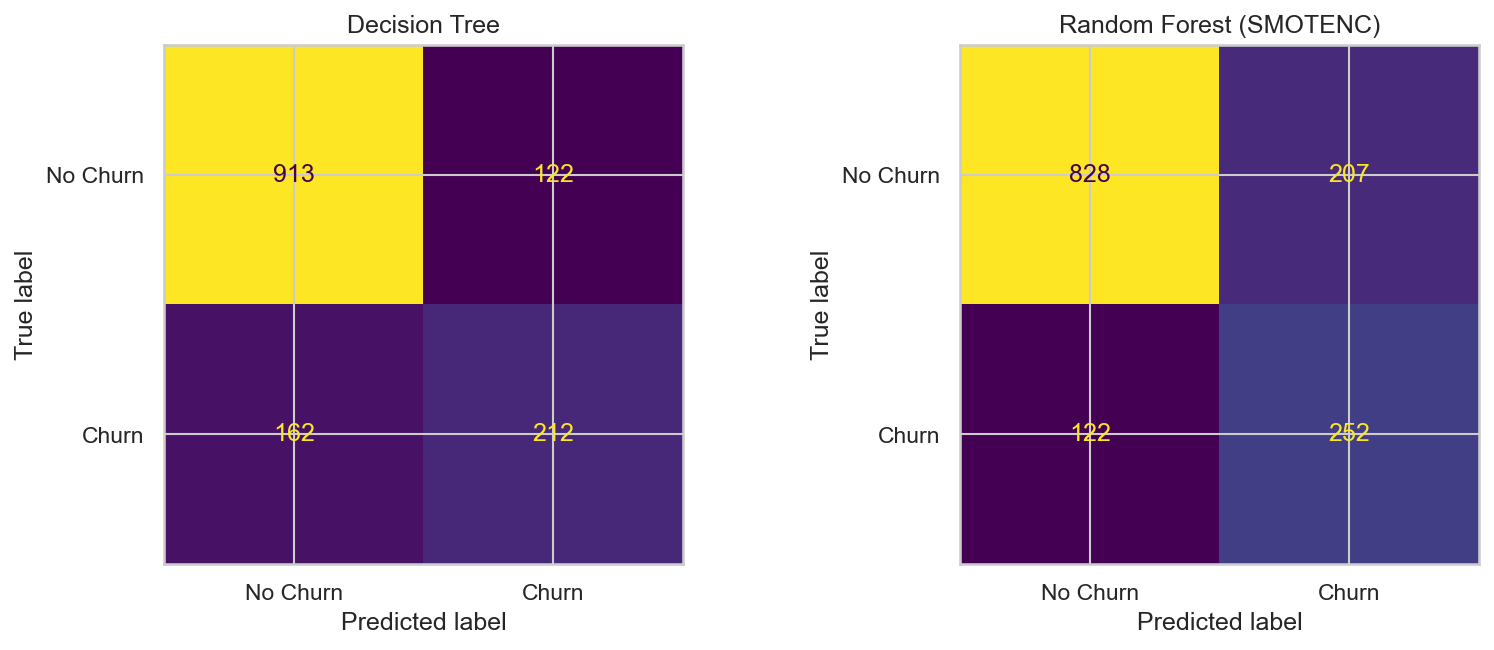
\includegraphics[width=0.48\textwidth]{figures_confusion_matrices.png}
		\caption{Confusion matrices for the best baseline model (Decision Tree, by F1) and the best SMOTENC model (Random Forest, by F1).}
		\label{fig:confmatrices}
	\end{figure}
	
	\begin{figure}[htbp]
		\centering
		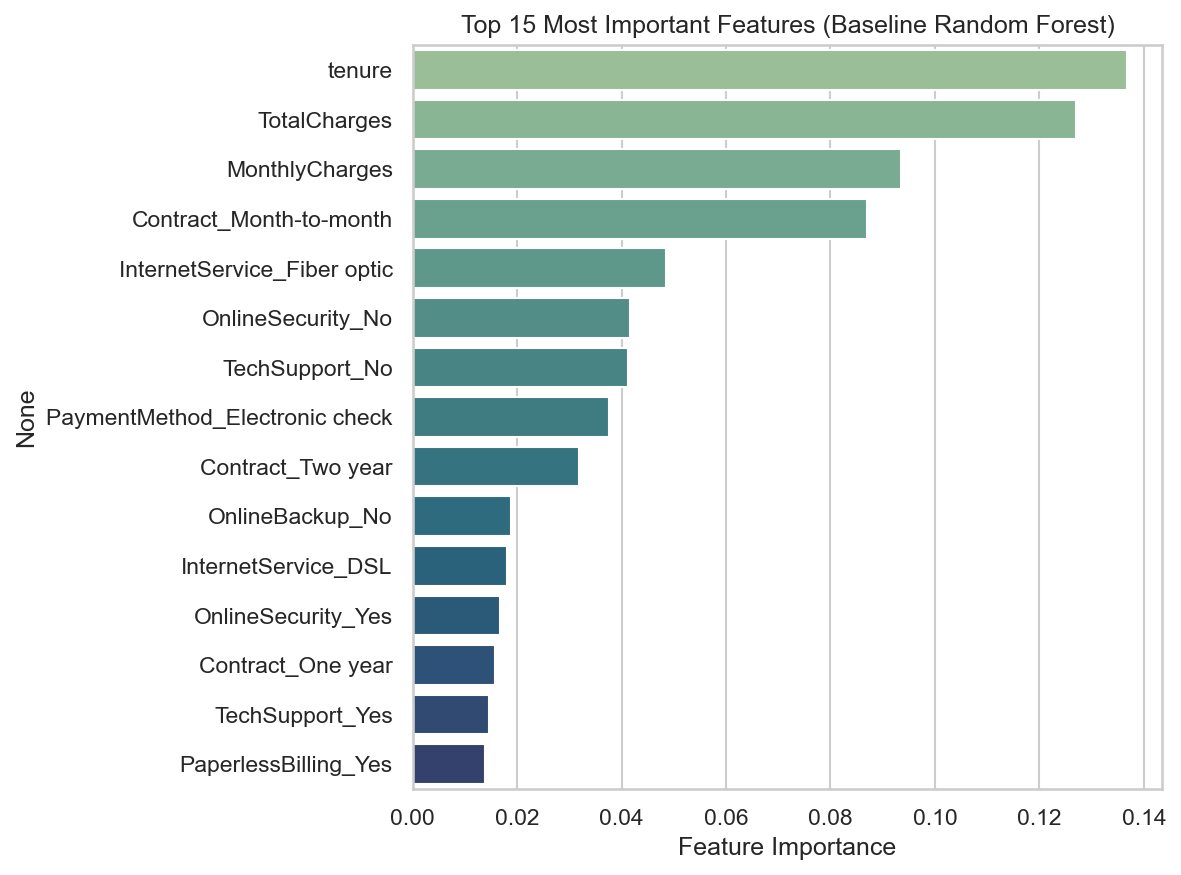
\includegraphics[width=0.48\textwidth]{figures_feature_importance.png}
		\caption{Top 15 features by importance, from the baseline Random Forest model.}
		\label{fig:featimportance}
	\end{figure}
	
	\subsection{Comparison of Approaches}
	The baseline Random Forest achieved the highest accuracy (80.3\%), ROC-AUC (0.839), and PR-AUC (0.653). Its precision was also the highest (66.2\%), but its churn recall was only 52.4\%, so it missed almost half of the actual churners. Baseline Naive Bayes showed the opposite behavior: it achieved the highest recall (81.0\%) but only 46.5\% precision. The baseline Decision Tree produced the highest baseline F1-score (0.599), balancing 63.5\% precision with 56.7\% recall.
	
	SMOTENC increased recall for Decision Tree, k-NN, and Random Forest, while Naive Bayes already had very high baseline recall and decreased slightly from 81.0\% to 77.8\%. In each algorithm family, the SMOTENC variant traded some accuracy or precision for higher minority-class sensitivity. Random Forest with SMOTENC achieved the highest F1-score (0.605), while Naive Bayes with SMOTENC was close at 0.603. Random Forest with SMOTENC offered higher precision (54.9\% versus 49.2\%), whereas Naive Bayes with SMOTENC offered higher recall (77.8\% versus 67.4\%). The small F1 difference means that a practical selection should be based on retention costs rather than ranking alone: Naive Bayes with SMOTENC favors catching more churners, whereas Random Forest with SMOTENC produces fewer false alarms. If probability ranking or minimizing unnecessary interventions is more important, the baseline Random Forest remains the strongest option because of its superior ROC-AUC, PR-AUC, and precision.
	
	\section{Discussion}
	\label{sec:discussion}
	
	\textit{Best-performing method.} No single algorithm dominated every metric. Random Forest's ensemble reduced the variance of a single Decision Tree and produced the strongest baseline ranking performance, as shown by both ROC-AUC and PR-AUC. However, using the default 0.5 decision threshold, it predicted the minority class conservatively and therefore had modest churn recall. SMOTENC shifted the Random Forest toward higher recall, although precision declined. Random Forest with SMOTENC achieved the highest F1-score, but its lead over Naive Bayes with SMOTENC was only 0.002. This difference is too small to justify a deployment decision by itself. A retention team should instead choose between these models using the relative business cost of a missed churner and an unnecessary offer.
	
	\textit{Limitations.} This study is based on a single dataset from one fictional telecom provider, so the results may not generalize to companies with different customer bases, pricing structures, or markets. Hyperparameter search was limited to small grids for tractability rather than an exhaustive or nested search. The final test set was used only after model selection, but a separate temporal or external validation set was unavailable, so performance on genuinely future customers remains unknown. SMOTENC avoids invalid interpolation across categorical codes, but its synthetic minority examples still depend on local patterns in the observed churners and may not represent all future churn behavior. Finally, the models were compared at the default 0.5 threshold rather than thresholds optimized for a known business cost.
	
	\textit{Observed model behavior.} Naive Bayes obtained high recall even though its conditional-independence assumption is not realistic for all attributes in this dataset. For example, several internet-service fields are related to one another. This result shows that a model with a simple assumption can still identify a large proportion of churn customers, although its lower precision means that it also produces more false alarms.
	
	\textit{Effect of data-quality issues.} The hidden \texttt{TotalCharges} issue occurred in only 11 of 7{,}043 records (0.16\%), so its effect was probably limited; however, this was not tested separately. It is still important because a standard null count did not reveal the blank strings. Class imbalance had a clearer effect on evaluation, as shown by the accuracy--recall trade-off between the baseline and SMOTENC variants.
	
	\textit{Ethical implications.} Demographic attributes were not among the most important Random Forest features in Fig.~\ref{fig:featimportance}, but this does not establish fairness. Before real use, performance and error rates should be checked across relevant customer groups.
	
	\section{Conclusion and Future Work}
	\label{sec:conclusion}
	
	This project compared Decision Tree, Gaussian Naive Bayes, k-NN, and Random Forest classifiers for predicting customer churn, with both baseline and SMOTENC training pipelines. The baseline Random Forest achieved the highest accuracy (80.3\%), precision (66.2\%), ROC-AUC (0.839), and PR-AUC (0.653). Random Forest with SMOTENC achieved the highest F1-score (0.605), with 67.4\% recall and 54.9\% precision. Naive Bayes with SMOTENC achieved a similar F1-score (0.603) and higher recall (77.8\%), but lower precision (49.2\%). The main practical conclusion is therefore not that one model is universally best. A high-recall retention campaign could prefer Naive Bayes with SMOTENC, while a campaign seeking to reduce unnecessary offers or rank customers reliably could prefer Random Forest. The Random Forest feature-importance analysis identifies which variables most influenced its predictions, but it does not establish the direction of those effects or a causal relationship with churn.
	
	Future work could compare additional algorithms such as Logistic Regression, Gradient Boosting, and XGBoost~\cite{b1}; test class weighting as an alternative to SMOTENC; and select decision thresholds using the actual costs of false positives and false negatives. Testing the models on data from another provider or a later time period would also show whether the results generalize.
	
	\section*{AI Tool Use and Originality Declaration}
	\label{sec:ai_declaration}
	
	Both ChatGPT and Claude were used for coding and debugging support and for improving the experimental pipeline. The student prepared the initial report outline, section structure, and content plan. ChatGPT assisted with developing parts of the report, locating literature candidates, language revision, structural refinement, and LaTeX formatting. The notebooks were executed, the numerical results were checked against the exported output, and the final wording, tables, figures, and citations were reviewed, verified, and revised by the student. The student accepts full responsibility for the accuracy, originality, reproducibility, and integrity of the submitted work.
	
	\begin{thebibliography}{00}
		
		\bibitem{b1} A.~K.~Ahmad, A.~Jafar, and K.~Aljoumaa, ``Customer churn prediction in telecom using machine learning in big data platform,'' \textit{Journal of Big Data}, vol.~6, no.~1, p.~28, 2019.
		
		\bibitem{b2} N.~Mustafa, L.~Sook Ling, and S.~F.~Abdul Razak, ``Customer churn prediction for telecommunication industry: A Malaysian case study,'' \textit{F1000Research}, vol.~10, p.~1274, 2021.
		
		\bibitem{b3} J.~K.~Sana, M.~Z.~Abedin, M.~S.~Rahman, and M.~S.~Rahman, ``A novel customer churn prediction model for the telecommunication industry using data transformation methods and feature selection,'' \textit{PLOS ONE}, vol.~17, no.~12, p.~e0278095, 2022.
		
		\bibitem{b4} N.~V.~Chawla, K.~W.~Bowyer, L.~O.~Hall, and W.~P.~Kegelmeyer, ``SMOTE: Synthetic minority over-sampling technique,'' \textit{Journal of Artificial Intelligence Research}, vol.~16, pp.~321--357, 2002.

		\bibitem{b5} S.~K.~Wagh, A.~A.~Andhale, K.~S.~Wagh, J.~R.~Pansare, S.~P.~Ambadekar, and S.~H.~Gawande, ``Customer churn prediction in telecom sector using machine learning techniques,'' \textit{Results in Control and Optimization}, vol.~14, p.~100342, 2024.

		\bibitem{b6} V.~Chang, K.~Hall, Q.~A.~Xu, F.~O.~Amao, M.~A.~Ganatra, and V.~Benson, ``Prediction of customer churn behavior in the telecommunication industry using machine learning models,'' \textit{Algorithms}, vol.~17, no.~6, p.~231, 2024.

		\bibitem{b7} IBM, ``Telco customer churn sample data,'' \textit{IBM Cognos Analytics Documentation}. [Online]. Available: \url{https://www.ibm.com/docs/en/cognos-analytics/12.0.x?topic=samples-telco-customer-churn}. Accessed: Jul.~28, 2026.

		\bibitem{b8} BlastChar, ``Telco Customer Churn,'' \textit{Kaggle}. [Online]. Available: \url{https://www.kaggle.com/datasets/blastchar/telco-customer-churn}. Accessed: Jul.~28, 2026.
		
	\end{thebibliography}
	
	\newpage	
	\appendix
	
	\section{Code Repository}
	\label{app:code}
	
	The source code, Jupyter notebooks, dependency list, results, and execution instructions are available at:
	
	\url{https://github.com/Bil-476-Project/Bil-476-Project}
	
	\section{Additional Figures and Tables}
	\label{app:additional}
	
	The main results table, F1-score comparison, ROC curves, precision--recall curves, confusion matrices, and feature-importance plot are included in Section~\ref{sec:results}. Table~\ref{tab:hyperparams} reports the best hyperparameters selected via stratified 5-fold cross-validation (optimizing F1-score). Baseline and SMOTENC variants were tuned independently.
	
	\begin{table}[htbp]
		\caption{Selected Hyperparameters (5-fold CV, optimizing F1)}
		\label{tab:hyperparams}
		\begin{center}
			\footnotesize
			\resizebox{\columnwidth}{!}{%
			\begin{tabular}{|l|l|c|}
				\hline
				\textbf{Model} & \textbf{Best Hyperparameters} & \textbf{CV F1} \\
				\hline
				Decision Tree & max\_depth=5, min\_samples\_leaf=10 & 0.565 \\
				\hline
				Naive Bayes & var\_smoothing=1e-7 & 0.599 \\
				\hline
				k-NN & n\_neighbors=21 & 0.591 \\
				\hline
				Random Forest & n\_estimators=200, max\_depth=10 & 0.578 \\
				\hline
				Decision Tree (SMOTENC) & max\_depth=3, min\_samples\_leaf=1 & 0.593 \\
				\hline
				Naive Bayes (SMOTENC) & var\_smoothing=1e-9 & 0.612 \\
				\hline
				k-NN (SMOTENC) & n\_neighbors=15 & 0.608 \\
				\hline
				Random Forest (SMOTENC) & n\_estimators=200, max\_depth=10 & 0.626 \\
				\hline
			\end{tabular}}
		\end{center}
	\end{table}
	
\end{document}
